% !TEX root = ../om_ts_01.tex

\begin{frame} % название фрагмента

\videotitle{Данные и задачи}

\end{frame}



\begin{frame}{Данные и задачи: план}
  \begin{itemize}[<+->]
    \item Временные ряды — тип данных.
    \item Задачи для одного ряда.
    \item Задачи для множества рядов. 
  \end{itemize}

\end{frame}


\begin{frame}{Заговор рептилоидов}

  \alert{Математический анализ:}

  \begin{block}{Последовательность}
    \[
      \frac{1}{2}, \frac{2}{3}, \frac{3}{4}, \frac{4}{5}, \ldots
    \]
  \end{block}
  
  \pause

  \begin{block}{Ряд}
    \[
      \frac{1}{2} + \frac{1}{4} + \frac{1}{8} +  \frac{1}{16} + \ldots
    \]
  \end{block}
  
  \pause

  Временные ряды — \alert{не ряды!}
\end{frame}
  



\begin{frame}{Что такое временной ряд?}

\begin{block}{Временной ряд}
Последовательность наблюдений, упорядоченных во времени. 
\[
0, 0, 5, 7, 102, 53, 23. 
\]
\end{block}

\pause
\begin{block}{Временной ряд}
Последовательность случайных величин, упорядоченных во времени. 
\[
y_1, y_2, y_3, y_4, \ldots, y_T.
\]
\end{block}
  

\end{frame}


\begin{frame}{Задачи для одного ряда}

\begin{itemize}[<+->]
  \item Спрогнозировать следующие значения.
  \item Восстановить пропущенные значения в середине ряда.
  \item Восстановить отдельные наблюдения по агрегированным.
  \item Обнаружить момент разладки.
  \item Выделить составляющие ряда. 
  \item \ldots 
\end{itemize}

\end{frame}


\begin{frame}{Прогнозируем}

  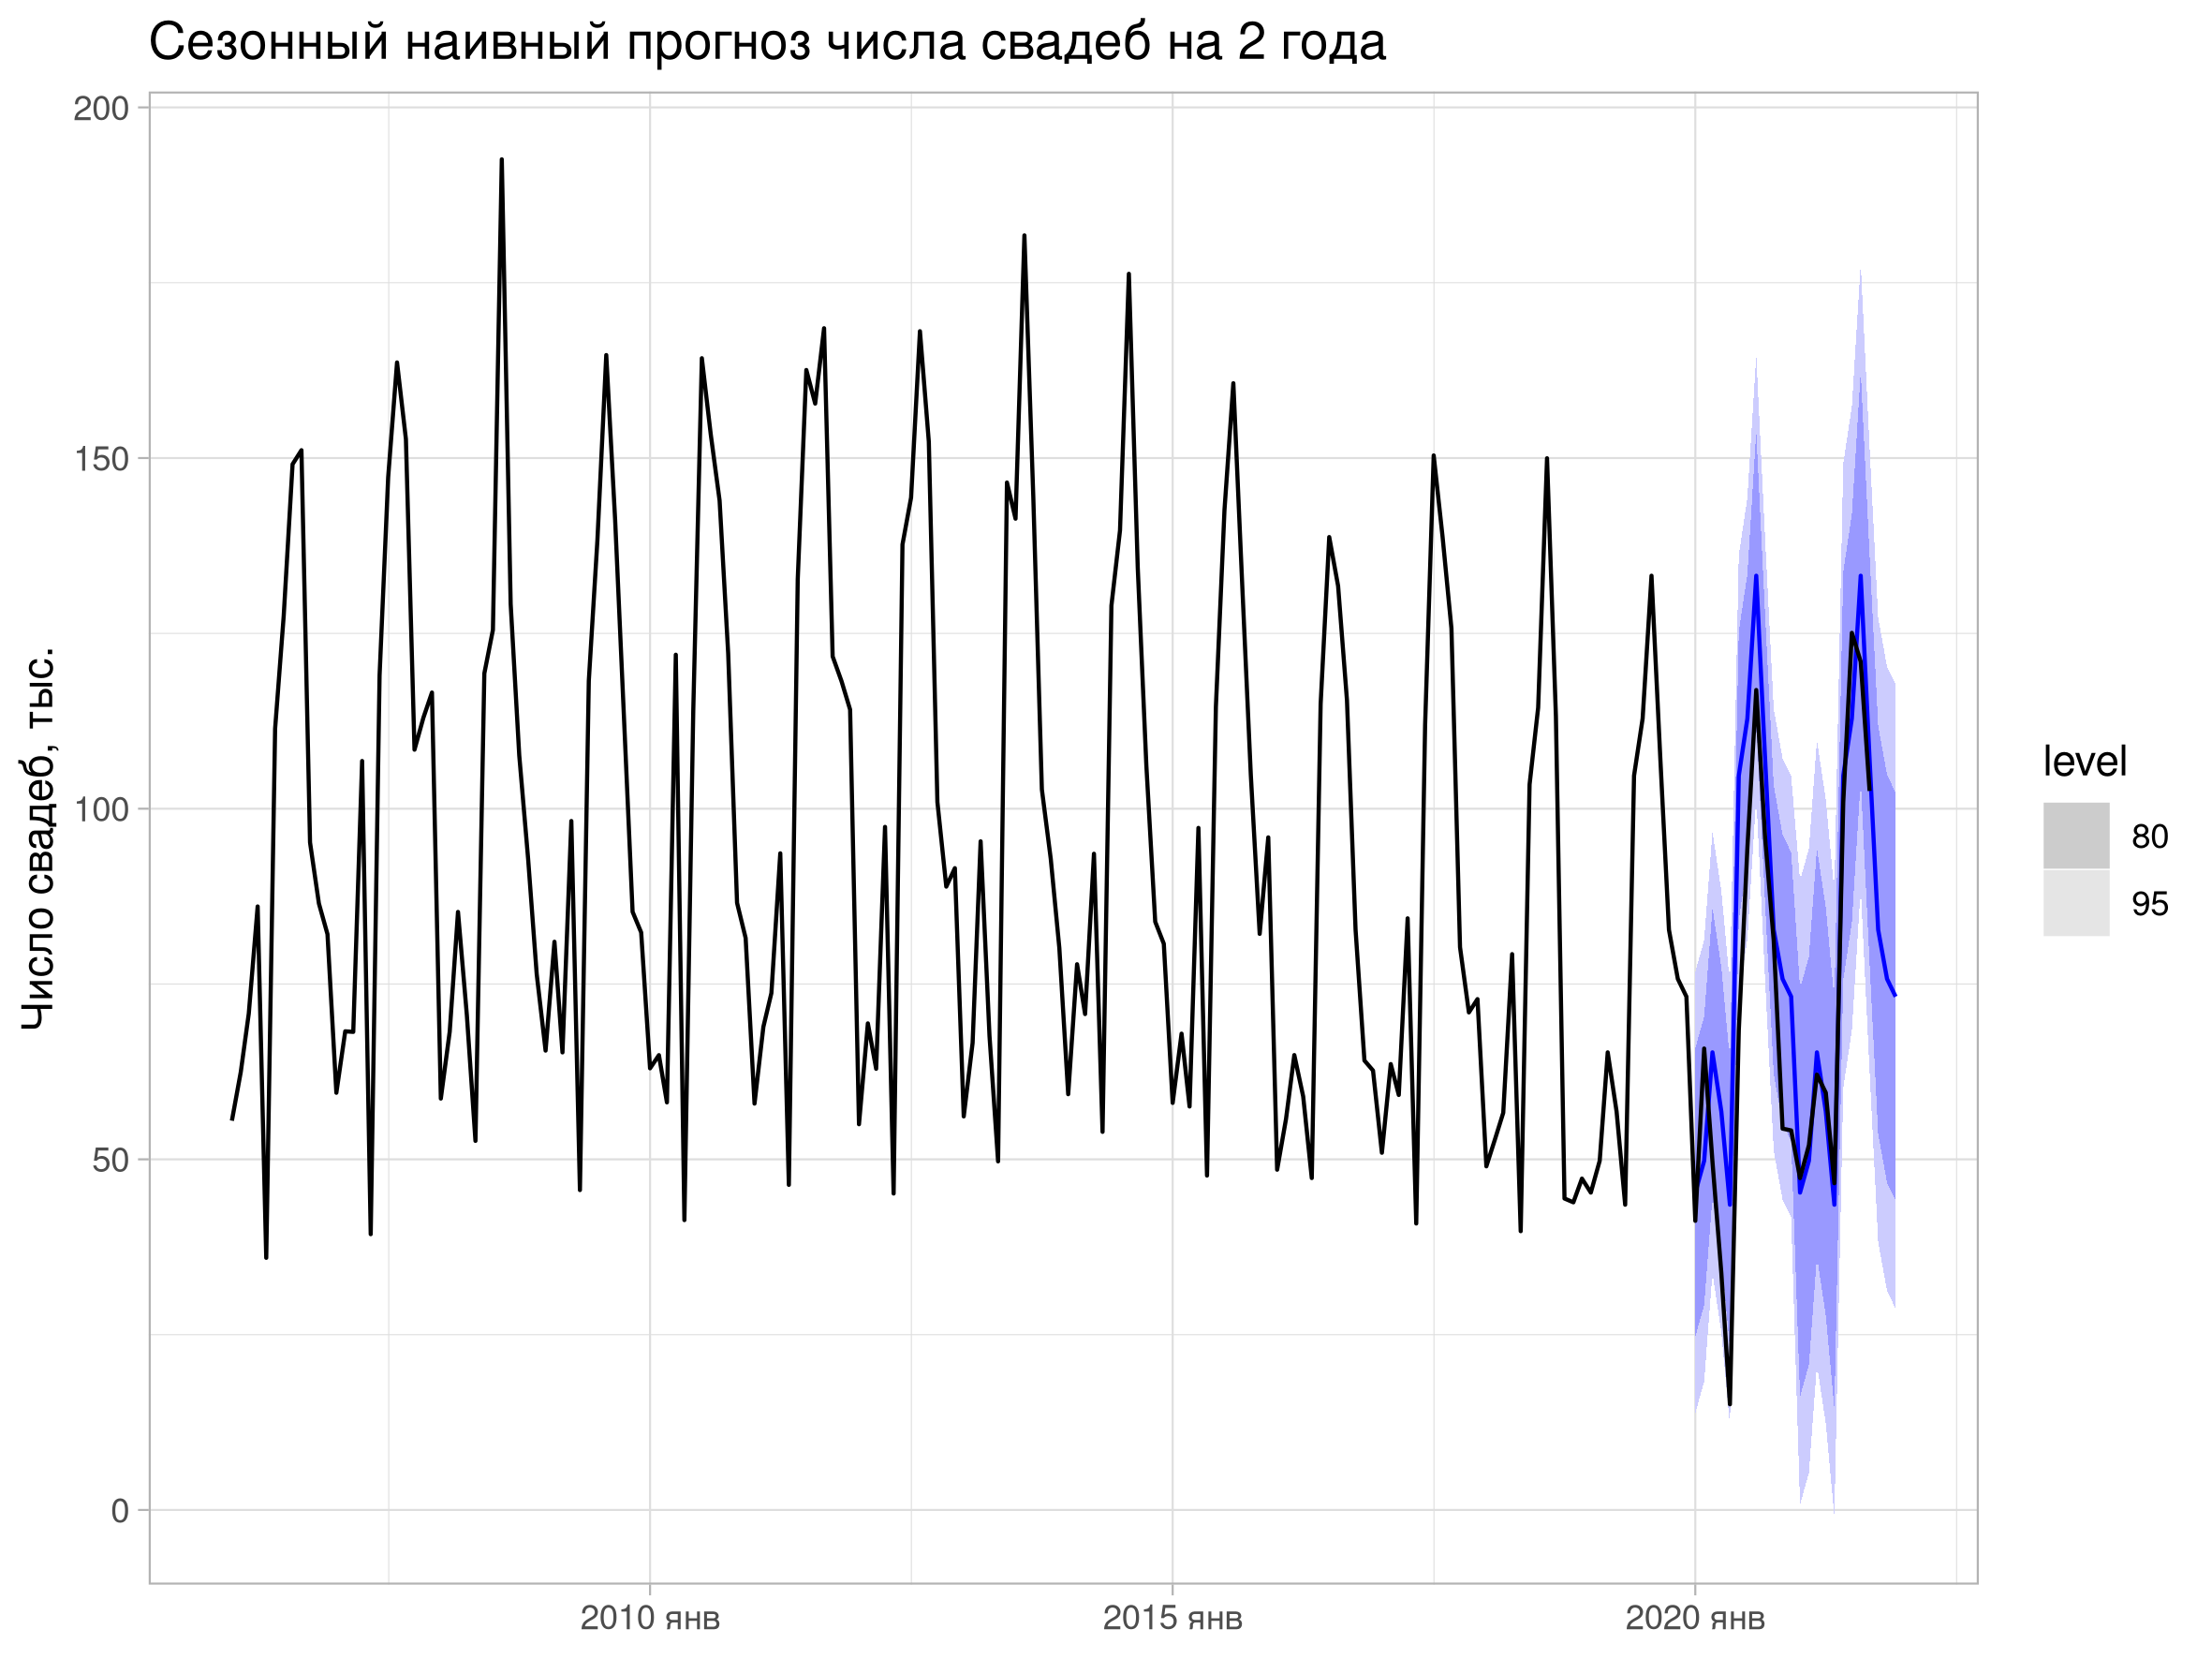
\includegraphics[width=\textwidth]{pictures/om_ts_01-017.png}

\end{frame}


\begin{frame}{Задачи для множества ряда}

  \begin{itemize}[<+->]
    \item Использовать дополнительные ряды при изучении целевого ряда.
    \item Понять, связаны ли ряды между собой.
    \item Измерить причинно-следственные связи.
    \item Классифицировать новый ряд в один из существующих классов.
    \item Понять, какие ряды близки к друг другу.
    \item Кластеризовать ряды на неизвестное множество кластеров.
    \item \ldots
  \end{itemize}
  
\end{frame}
  
\begin{frame}{Измеряем близость рядов}

  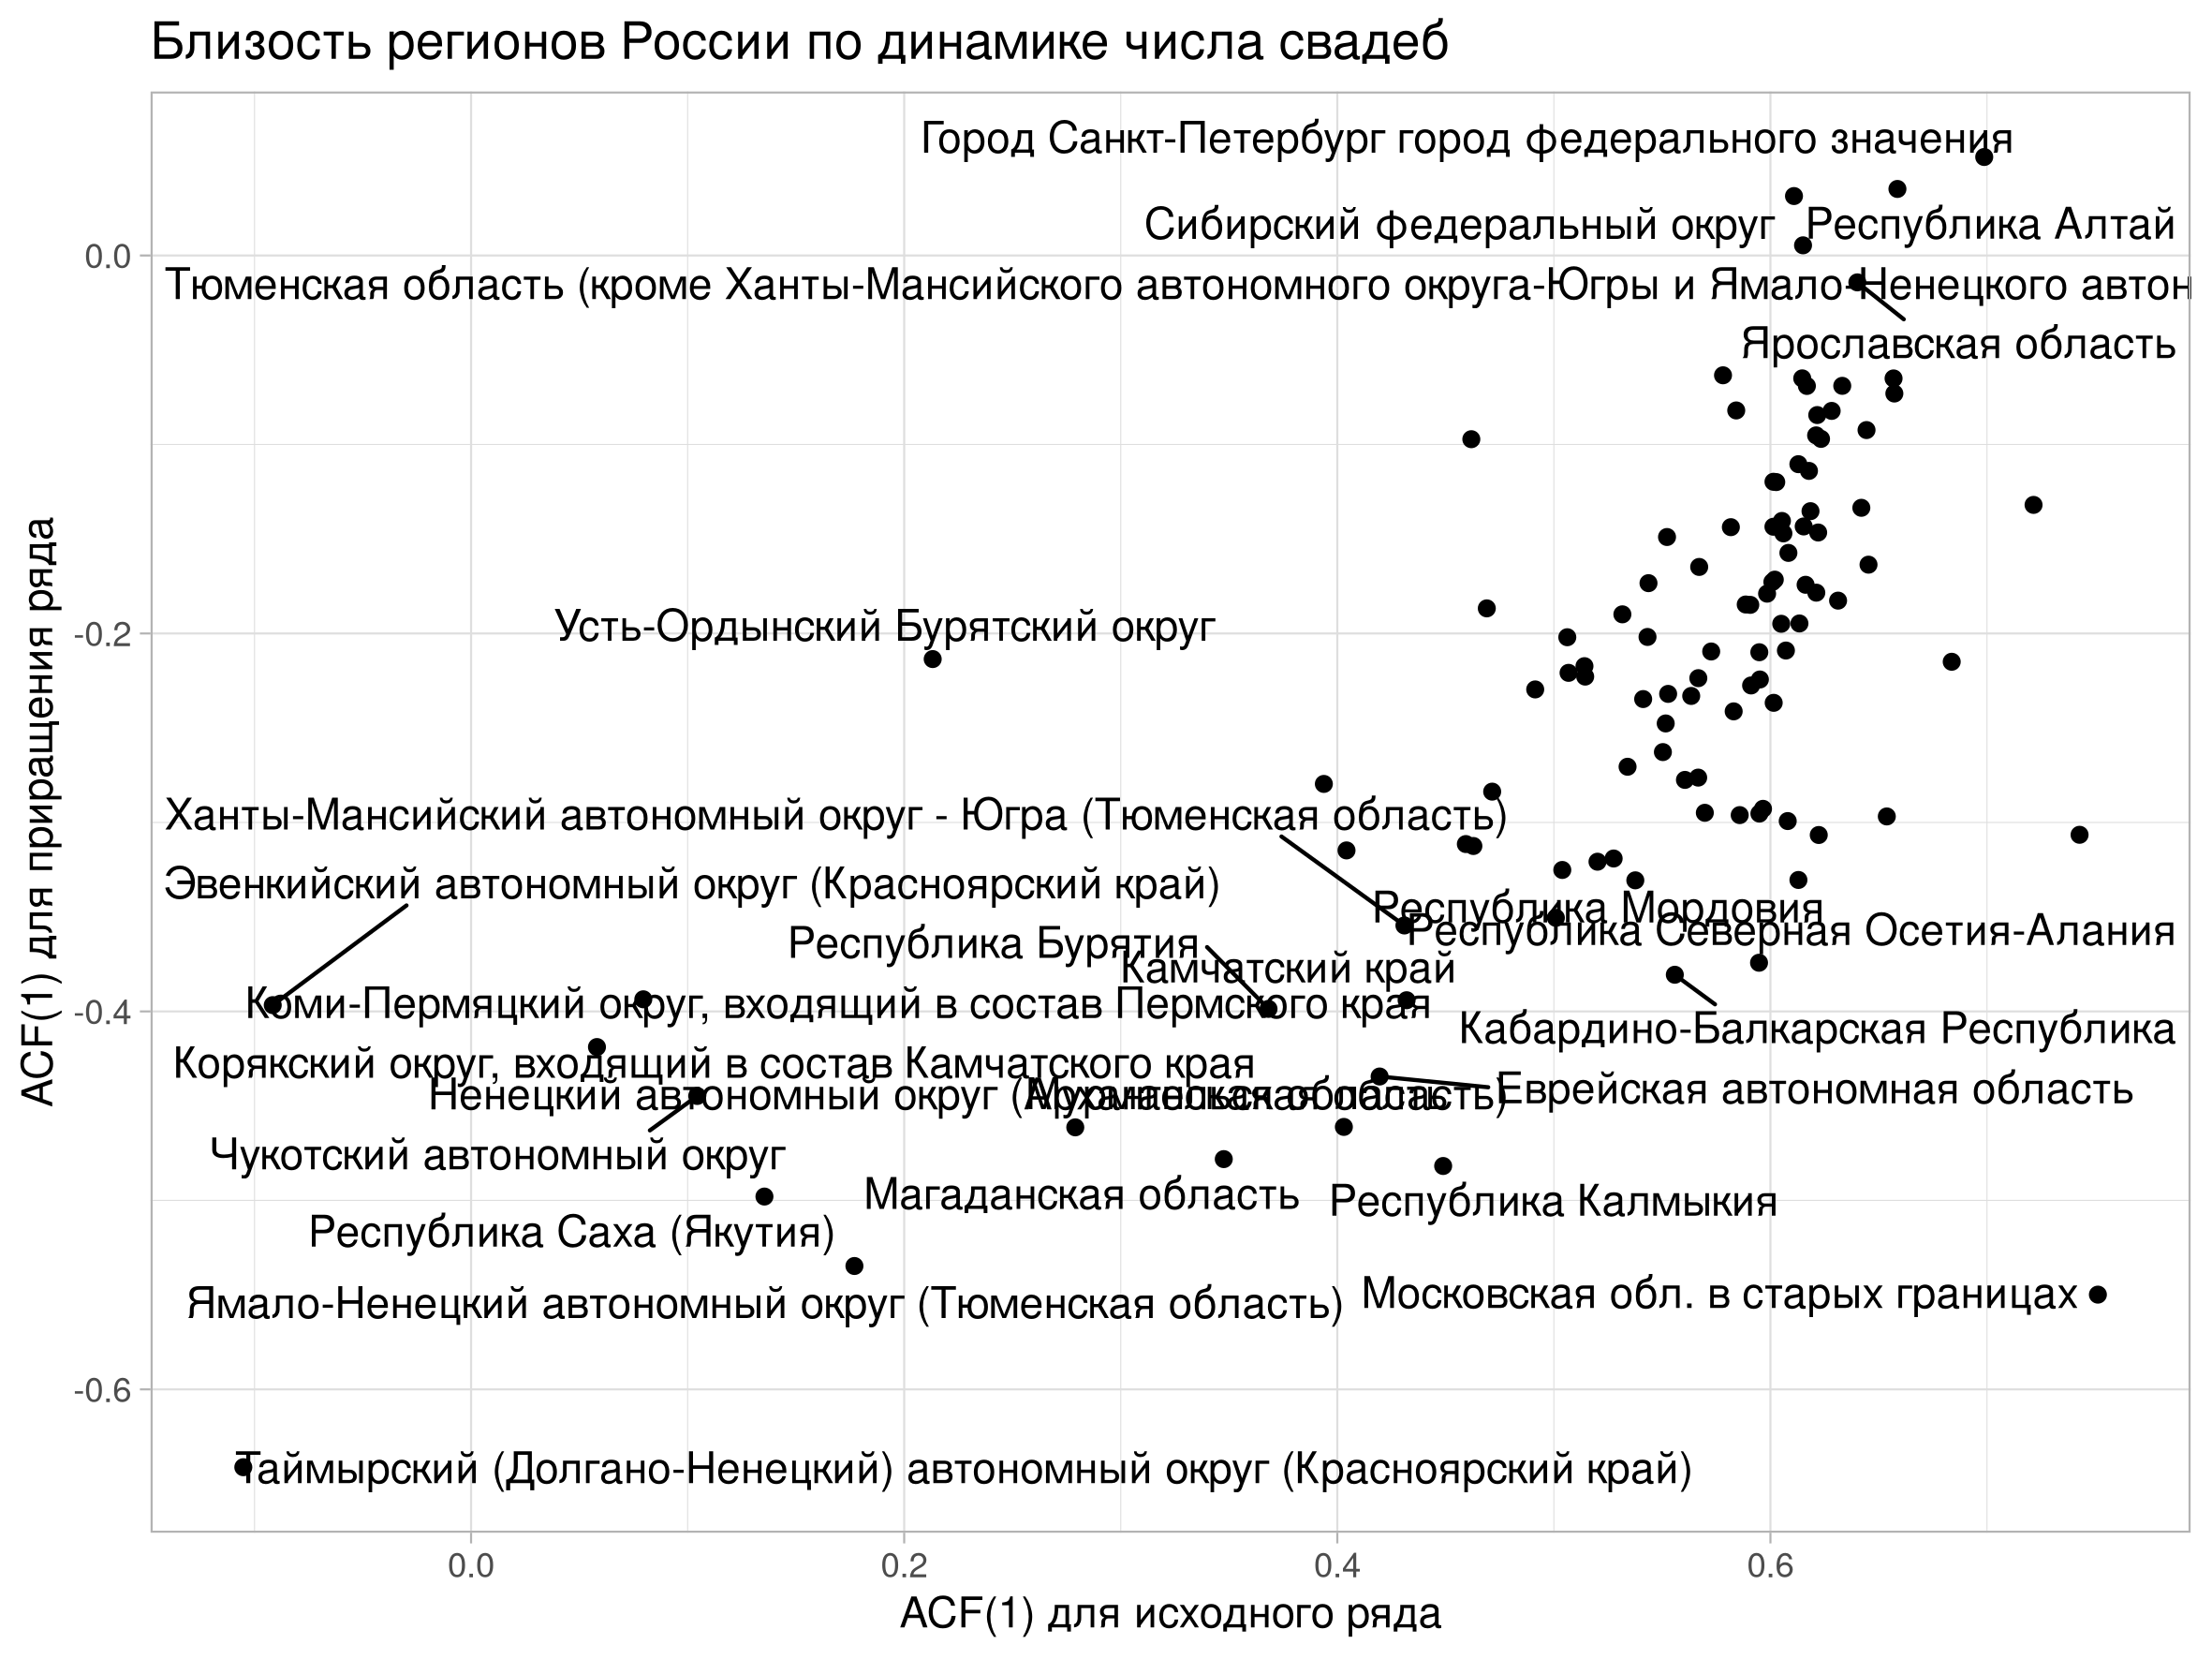
\includegraphics[width=\textwidth]{pictures/om_ts_01-025.png}


\end{frame}



\begin{frame}{Модели и алгоритмы}

\begin{block}{Модели}
\begin{itemize}[<+->]
  \item Явные предположения про величины $y_1$, $y_2$, \ldots, $y_T$.
  \item Метод оценивания: максимальное правдоподобие, байесовский подход.
  \item Точечные и интервальные прогнозы, проверка гипотез. 
\end{itemize}
\end{block}

ETS, ARIMA, ORBIT, PROPHET, \ldots

\end{frame}

\begin{frame}{Модели и алгоритмы}

\begin{block}{Алгоритмы}
  \begin{itemize}[<+->]
    \item Размытые предположения про величины $y_1$, $y_2$, \ldots, $y_T$.
    \item Особая инструкция.
    \item Точечные результаты без доверительных интервалов. 
  \end{itemize}
\end{block}
  
STL, градиентный бустинг, случайный лес, \ldots

\end{frame}

\begin{frame}{Фокус курса}

Прогнозирование одномерных рядов с помощью моделей. 

\end{frame}



